\subsection{LQR を平方完成で導く}

極配置では、閉ループ極を指定して応答の速さや減衰を設計した。しかし、台車の位置をすばやく戻したい一方で加える力には上限がある、あるいはモータの角度誤差を小さくしたい一方で電流を大きくしすぎたくない、という設計では、極だけでは「状態のずれ」と「入力の大きさ」をどの割合で許すかを数値で比較できない。極を速く置けば偏差は早く消えるが、一般に入力は大きくなり、飽和や発熱の制約に近づく。そこで、状態偏差を二次形式 $x^\T Qx$、入力努力を $u^\T Ru$ として同じ評価関数へ入れ、重み $Q,R$ によってその交換条件を明示する。平方完成は、この二次評価の中で入力 $u$ がどの値を選ぶと残りコストを最も小さくするかを直接取り出すために用いる。

\begin{theorem}[連続時間 LQR のリカッチ方程式]
$(A,B)$ が可安定で、$(A,Q^{1/2})$ が可検出である線形系 $\dot{x}=Ax+Bu$ に対し、評価関数
\begin{equation}
  J=\int_0^\infty (x^\T Qx+u^\T Ru)\,\dd t,
  \qquad Q=Q^\T\ge0,
  \quad R=R^\T>0
\end{equation}
を最小にする状態フィードバックは
\begin{equation}
  u=-R^{-1}B^\T Px
\end{equation}
であり、$P$ は代数リカッチ方程式
\begin{equation}
  A^\T P+PA-PBR^{-1}B^\T P+Q=0
\end{equation}
を満たす半正定値の安定化解である。
\end{theorem}

\begin{derivation}
最適な残りコストが二次形式
\begin{equation}
  V(x)=x^\T Px
\end{equation}
で表せると仮定する。最適制御の動的計画法、すなわち Hamilton--Jacobi--Bellman 方程式より
\begin{equation}
  0=\min_u\{x^\T Qx+u^\T Ru+\dot{V}(x)\}
\end{equation}
である。$\dot{x}=Ax+Bu$ なので
\begin{align}
  \dot{V}
  &=\dot{x}^\T Px+x^\T P\dot{x}\\
  &=(Ax+Bu)^\T Px+x^\T P(Ax+Bu)\\
  &=x^\T A^\T Px+u^\T B^\T Px+x^\T PAx+x^\T PBu.
\end{align}
スカラーは転置しても同じなので $u^\T B^\T Px=x^\T PBu$ である。したがって
\begin{equation}
  \dot{V}=x^\T(A^\T P+PA)x+2u^\T B^\T Px.
\end{equation}
HJB 方程式の中身は
\begin{equation}
  x^\T Qx+x^\T(A^\T P+PA)x+u^\T Ru+2u^\T B^\T Px
\end{equation}
である。$u$ に関する部分を平方完成する。
\begin{align}
  u^\T Ru+2u^\T B^\T Px
  &=(u+R^{-1}B^\T Px)^\T R(u+R^{-1}B^\T Px)\\
  &\quad -x^\T PBR^{-1}B^\T Px.
\end{align}
第一項は $R>0$ より非負であり、最小にするには
\begin{equation}
  u+R^{-1}B^\T Px=0
\end{equation}
とすればよい。よって
\begin{equation}
  u=-R^{-1}B^\T Px
\end{equation}
である。残りの $x$ に関する項が任意の $x$ で 0 になる必要があるので
\begin{equation}
  A^\T P+PA-PBR^{-1}B^\T P+Q=0
\end{equation}
を得る。
\end{derivation}

\subsection{有限ホライズン LQR とリカッチ微分方程式}

無限ホライズン LQR では、残り時間がいつも無限にあるため、最適な残りコスト $V(x)=x^\T Px$ は時刻に依存しなかった。有限ホライズンでは事情が変わる。終端時刻 $T$ が近づけば、入力を使って状態を戻す余裕が少なくなるので、同じ状態 $x$ に対する「残りコスト」は現在時刻 $t$ によって変わる。したがって、値関数は
\begin{equation}
  V(t,x)=\min_{u(\cdot)}
  \left\{
    x(T)^\T S x(T)
    +\int_t^T
      \left(x(\tau)^\T Qx(\tau)+u(\tau)^\T Ru(\tau)\right)\,\dd \tau
  \right\}
  \label{eq:finite-lqr-value}
\end{equation}
と書く。状態は $x(t)\in\R^n$、入力は $u(t)\in\R^m$、システムは
\begin{equation}
  \dot{x}(\tau)=Ax(\tau)+Bu(\tau),
  \qquad x(t)=x
\end{equation}
である。ここでは $A,B,Q,R,S$ は時不変とし、$Q=Q^\T\ge0$、$R=R^\T>0$、$S=S^\T\ge0$ を仮定する。$Q$ は途中の状態偏差を罰する重み、$R$ は途中の入力の大きさを罰する重み、$S$ は終端時刻に残った状態偏差を罰する重みである。単位を持つ物理量を扱うときは、$x^\T Qx$、$u^\T Ru$、$x(T)^\T S x(T)$ が同じ「評価関数の単位」になるように重みを選ぶ。$Q$ を大きくすると途中のずれを嫌い、$R$ を大きくすると入力を節約し、$S$ を大きくすると終端で原点や目標偏差へ近づけることを強く求める。後の MPC の記号では、この終端重みを $P_f$ と書くことが多い。

図\ref{fig:flow45-lqr-horizon-examples}は、導出に入る前に有限ホライズンの予測、重みの交換条件、後退リカッチ計算の意味を同じ二重積分器で並べたものである。サンプル周期 $h=0.1\,\mathrm{s}$ とし、状態を位置偏差と速度偏差、入力を台車へ加える正規化力とみなす。左上では終端重みを $S_N=0$ とした予測を、$N=8,16,32$ サンプルで描いている。短いホライズンでは、予測区間の外側に残る状態を評価できないため、終端近くで入力を弱めたまま大きな位置偏差を残す。ホライズンを長くすると、同じ初期偏差に対して先の状態偏差まで費用に入るので、早い段階から状態を戻す入力が選ばれる。

\begin{figure}[tb]
\centering
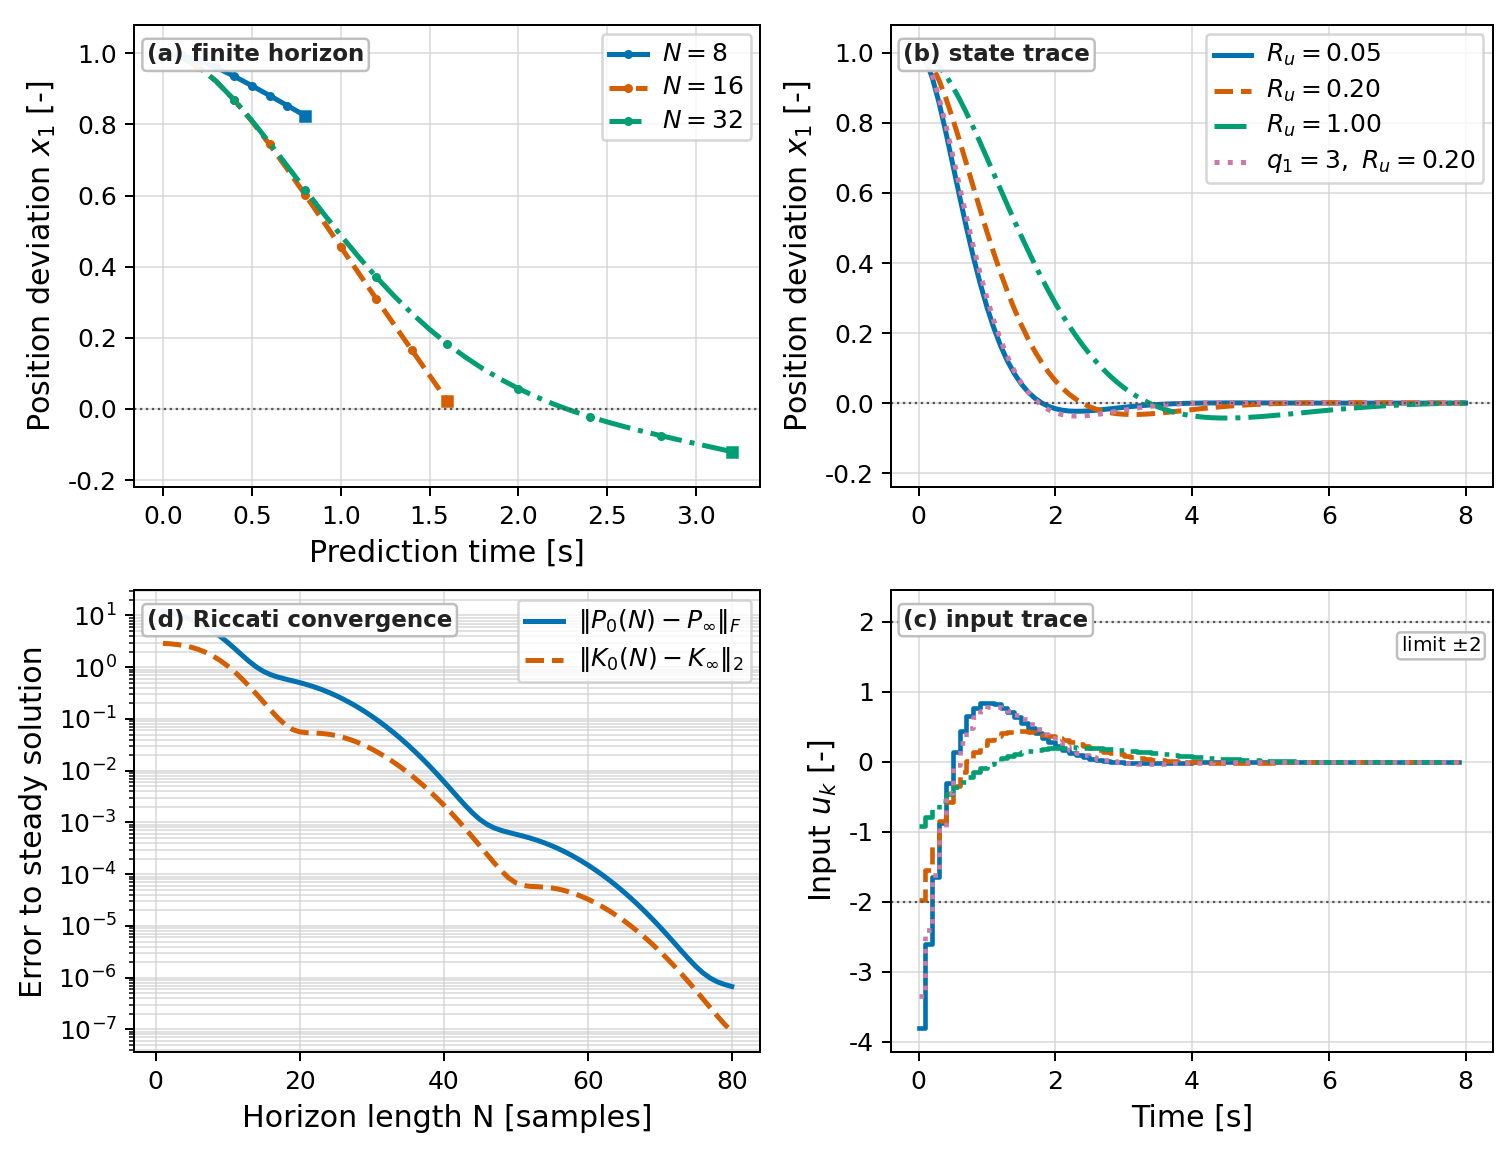
\includegraphics[width=0.96\linewidth,bb=0 0 1512 1152]{figures/flow45_lqr_horizon_examples.png}
\caption{有限ホライズン LQR における予測、重み掃引、後退リカッチ収束の例。二重積分器で予測ホライズン $N$ を変えると、予測区間内に含まれる将来偏差が変わる。入力重み $R_u$ や位置重み $q_1$ を変えると、位置偏差の整定、入力努力、入力限界 $\pm 2$ に対する制約余裕が同時に変わる。左下は $S_N=0$ から後退リカッチ再帰を始めても、ホライズンを長くすると現在時刻の $P_0(N)$ と $K_0(N)$ が定常解 $P_\infty,K_\infty$ へ近づくことを示す。}
\label{fig:flow45-lqr-horizon-examples}
\end{figure}

右上と右下は、各時刻で同じ有限ホライズン問題を解き、最初の入力だけを使ったときの状態と入力の履歴である。$Q_x=\diag(1,0.08)$ のまま $R_u=0.05$ と小さくすると、位置偏差は約 $2.7\,\mathrm{s}$ で零近傍へ入るが、最大入力は約 $3.8$ となり、入力限界 $\pm 2$ に対する制約余裕は約 $-1.8$ である。これは、理想的な線形 LQR が要求する入力が実機の限界を越えていることを意味する。反対に $R_u=1.00$ と大きくすると、最大入力は約 $0.9$ に抑えられ、制約余裕は約 $1.1$ 残るが、整定は約 $6.1\,\mathrm{s}$ まで遅くなる。$R_u=0.20$ のまま位置重みを $q_1=3$ に増やした場合も整定は速くなる一方で、最大入力は約 $3.4$ となり、制約余裕は負になる。したがって、状態重みを大きくすることと入力重みを小さくすることは、どちらも状態偏差を早く減らす方向に働くが、入力努力と飽和余裕を同時に消費する。制約を評価関数に入れていない LQR では、点線の入力限界は最適化の制約ではなく実装上の監視線であり、限界を越える設計は飽和、アンチワインドアップ、または後の MPC のような制約付き予測制御で再評価する必要がある。

左下の曲線は、有限ホライズンの後退リカッチ再帰が無限ホライズン LQR へ近づく仕組みを表す。終端条件を $S_N=0$ としても、$N$ が長くなると現在時刻から終端までに十分な将来コストが積み上がり、$P_0(N)$ と最初のゲイン $K_0(N)$ は代数リカッチ方程式の安定化解から得られる $P_\infty,K_\infty$ へ近づく。つまり、有限ホライズン LQR の時刻依存ゲインは、終端の近くでは終端重みの影響を強く受けるが、終端から十分離れた区間では定常 LQR とほぼ同じ振る舞いになる。この観察が、次の HJB 方程式で時刻依存の $P(t)$ を導入し、その後で $\dot{P}=0$ の定常解を取り出す理由である。

動的計画法では、時刻 $t$ で少しだけ進んだ後も、残り区間では同じ形の最適化問題を解くと考える。連続時間の Hamilton--Jacobi--Bellman 方程式は
\begin{equation}
  0=\min_u
  \left\{
    x^\T Qx+u^\T Ru
    +\partial_t V(t,x)
    +\partial_x V(t,x)^\T(Ax+Bu)
  \right\}
  \label{eq:finite-lqr-hjb}
\end{equation}
であり、終端条件は
\begin{equation}
  V(T,x)=x^\T S x
  \label{eq:finite-lqr-terminal-value}
\end{equation}
である。線形系と二次評価関数の組では、値関数も二次形式になると予想できるので
\begin{equation}
  V(t,x)=x^\T P(t)x,
  \qquad P(t)=P(t)^\T
  \label{eq:finite-lqr-ansatz}
\end{equation}
と置く。この形を仮定して HJB 方程式へ代入し、最後にその仮定が閉じていることを確かめる。まず
\begin{align}
  \partial_t V(t,x)&=x^\T \dot{P}(t)x,\\
  \partial_x V(t,x)&=2P(t)x
\end{align}
である。したがって
\begin{align}
  \partial_x V^\T(Ax+Bu)
  &=2x^\T P(t)Ax+2x^\T P(t)Bu\\
  &=x^\T\{A^\T P(t)+P(t)A\}x+2u^\T B^\T P(t)x
\end{align}
となる。二つ目の等号では、$x^\T P A x$ がスカラーであり、転置して $x^\T A^\T P x$ と足し合わせられることを使った。

\weq{finite-lqr-hjb} の中で $u$ に依存する部分は
\begin{equation}
  u^\T Ru+2u^\T B^\T P(t)x
\end{equation}
である。これは前の無限ホライズン LQR と同じ平方完成で
\begin{align}
  u^\T Ru+2u^\T B^\T P(t)x
  &=
  \left(u+R^{-1}B^\T P(t)x\right)^\T
  R
  \left(u+R^{-1}B^\T P(t)x\right)\\
  &\quad
  -x^\T P(t)BR^{-1}B^\T P(t)x
\end{align}
と整理できる。$R>0$ なので第一項は非負であり、最小値は
\begin{equation}
  u^*(t)=-R^{-1}B^\T P(t)x(t)
  \label{eq:finite-lqr-control}
\end{equation}
で達成される。したがって有限ホライズン LQR のフィードバックゲインは
\begin{equation}
  K(t)=R^{-1}B^\T P(t)
  \label{eq:finite-lqr-gain}
\end{equation}
であり、一般には時刻によって変わる。

最小化後の HJB 方程式に残る $x$ の二次形式は
\begin{equation}
  x^\T
  \left\{
    \dot{P}
    +A^\T P+PA
    -PBR^{-1}B^\T P
    +Q
  \right\}
  x=0
\end{equation}
である。これは任意の $x$ で成り立たなければならないので、行列の係数が 0 になる。よって有限ホライズン連続時間 LQR のリカッチ微分方程式
\begin{equation}
  -\dot{P}(t)
  =
  A^\T P(t)+P(t)A
  -P(t)BR^{-1}B^\T P(t)
  +Q,
  \qquad P(T)=S
  \label{eq:finite-lqr-rde}
\end{equation}
を得る。右端の $P(T)=S$ は初期条件ではなく終端条件である。したがって、数値計算では $t=T$ から $t=0$ へ向かって逆向きに解くか、残り時間 $\sigma=T-t$ を導入して前向きの微分方程式として解く。$P(t)$ が得られれば、各時刻で \weq{finite-lqr-control} を用いるだけでよい。

同じ式は Hamiltonian の最適性条件からも確認できる。Hamiltonian を
\begin{equation}
  \mathcal{H}(x,u,\lambda)
  =x^\T Qx+u^\T Ru+\lambda^\T(Ax+Bu)
\end{equation}
と置くと、最適性条件は
\begin{align}
  0&=\frac{\partial \mathcal{H}}{\partial u}
    =2Ru+B^\T\lambda,\\
  -\dot{\lambda}&=\frac{\partial \mathcal{H}}{\partial x}
    =2Qx+A^\T\lambda,\\
  \lambda(T)&=2Sx(T)
\end{align}
である。値関数から得られる関係 $\lambda=\partial_x V=2P(t)x$ を代入すると
\begin{equation}
  u^*=-\frac{1}{2}R^{-1}B^\T\lambda
  =-R^{-1}B^\T P(t)x
\end{equation}
となる。さらに
\begin{align}
  \dot{\lambda}
  &=2\dot{P}x+2P\dot{x}\\
  &=2\dot{P}x+2P(Ax-BR^{-1}B^\T Px)
\end{align}
である。これを随伴方程式 $-\dot{\lambda}=2Qx+2A^\T Px$ と比べれば
\begin{equation}
  \dot{P}+A^\T P+PA-PBR^{-1}B^\T P+Q=0
\end{equation}
が再び得られる。動的計画法では「残りコスト」を直接扱い、Hamiltonian 形式では「状態の変化に対するコストの感度」である随伴変数を扱うが、LQR では両者が $\lambda=2Px$ で同じ内容に結びつく。

前の平方完成による無限ホライズン LQR は、有限ホライズンの式から $\dot{P}=0$ となる定常解を取り出したものと見られる。残り時間が十分長く、$(A,B)$ が可安定で $(A,Q^{1/2})$ が可検出なら、$P(t)$ は多くの場合、区間の内側で代数リカッチ方程式の安定化解 $P_\infty$ に近づく。すなわち
\begin{equation}
  A^\T P_\infty+P_\infty A
  -P_\infty BR^{-1}B^\T P_\infty+Q=0
\end{equation}
であり、$K_\infty=R^{-1}B^\T P_\infty$ が時間不変ゲインになる。

有限ホライズンの終端重み $S$ は、後で扱う MPC の終端コストと同じ役割を持つ。MPC では制約を含むため、各サンプル時刻で有限ホライズン問題を解き直し、最初の入力だけを使う。ホライズンの先をまったく考えないと、予測区間の終わりで不自然な入力や状態が選ばれることがある。そのため終端コスト $V_f(x)=x^\T P_f x$ を置き、$P_f$ に LQR のリカッチ解を使う。これは、予測区間の外側で局所 LQR を続けたときの残りコストを有限ホライズン問題の末端へ折り込む操作である。

\subsection{離散時間 LQR と代数リカッチ方程式}

デジタル制御器では、入力はサンプリング時刻ごとに更新される。サンプリング周期を $h>0$ とし、零次ホールドや数値積分により得られた離散時間モデルを
\begin{equation}
  x_{k+1}=A_d x_k+B_d u_k
  \label{eq:dlqr-system}
\end{equation}
と書く。ここで $x_k\in\R^n$ は時刻 $kh$ の状態偏差、$u_k\in\R^m$ は区間 $[kh,(k+1)h)$ で保持される入力偏差であり、$A_d\in\R^{n\times n}$、$B_d\in\R^{n\times m}$ はサンプル周期を含む行列である。以下では、$A_d,B_d$ は時不変、初期状態 $x_0$ は既知、入力には明示的な上下限制約がないと仮定する。重み行列は
\begin{equation}
  Q_x=Q_x^\T\ge0,
  \qquad
  R_u=R_u^\T>0,
  \qquad
  S_N=S_N^\T\ge0
\end{equation}
とし、有限ホライズン評価関数を
\begin{equation}
  J_N
  =
  x_N^\T S_N x_N
  +\sum_{k=0}^{N-1}
  \left(x_k^\T Q_x x_k+u_k^\T R_u u_k\right)
  \label{eq:dlqr-finite-cost}
\end{equation}
で定める。$Q_x$ はサンプル時刻での状態偏差、$R_u$ は入力の大きさ、$S_N$ はホライズン末端の状態偏差を評価する。連続時間評価を離散化して対応させる場合、単純な近似では $Q_x\simeq hQ_c$、$R_u\simeq hR_c$ と置くが、実際には $A_d,B_d$ も $h$ に依存するため、サンプリング周期を変えたときは重みとゲインを同時に再評価する。

動的計画法により、時刻 $k$ から終端までの最小残りコストを
\begin{equation}
  V_k(x)=x^\T P_k x,
  \qquad P_k=P_k^\T
  \label{eq:dlqr-value}
\end{equation}
と置く。終端条件は
\begin{equation}
  P_N=S_N
  \label{eq:dlqr-terminal}
\end{equation}
である。時刻 $k$ では
\begin{align}
  V_k(x)
  =
  \min_u
  \{x^\T Q_x x+u^\T R_u u
  +(A_d x+B_d u)^\T P_{k+1}(A_d x+B_d u)\}
  \label{eq:dlqr-bellman}
\end{align}
が成り立つ。\weq{dlqr-bellman} の中身を展開すると
\begin{align}
  &x^\T(Q_x+A_d^\T P_{k+1}A_d)x\\
  &\quad
  +2u^\T B_d^\T P_{k+1}A_d x
  +u^\T(R_u+B_d^\T P_{k+1}B_d)u
  \label{eq:dlqr-expanded}
\end{align}
となる。$P_{k+1}\ge0$ なら
\begin{equation}
  H_k=R_u+B_d^\T P_{k+1}B_d
  \label{eq:dlqr-hessian}
\end{equation}
は正定値である。したがって、$u$ に関する二次式は平方完成により
\begin{align}
  &u^\T H_k u+2u^\T B_d^\T P_{k+1}A_d x\\
  &=
  (u+H_k^{-1}B_d^\T P_{k+1}A_d x)^\T
  H_k
  (u+H_k^{-1}B_d^\T P_{k+1}A_d x)\\
  &\quad
  -x^\T A_d^\T P_{k+1}B_d
  H_k^{-1}
  B_d^\T P_{k+1}A_d x
  \label{eq:dlqr-completion}
\end{align}
と整理できる。第一項は非負であり、最小値は
\begin{equation}
  u_k^*=-K_kx_k
  \label{eq:dlqr-optimal-input}
\end{equation}
で達成される。ここで有限ホライズンの離散時間 LQR ゲインは
\begin{equation}
  K_k
  =
  (R_u+B_d^\T P_{k+1}B_d)^{-1}
  B_d^\T P_{k+1}A_d
  \label{eq:dlqr-finite-gain}
\end{equation}
である。最小化後の $x$ の二次形式を $x^\T P_kx$ と同一視すると、後退リカッチ再帰
\begin{equation}
  P_k
  =
  Q_x+A_d^\T P_{k+1}A_d
  -A_d^\T P_{k+1}B_d
  (R_u+B_d^\T P_{k+1}B_d)^{-1}
  B_d^\T P_{k+1}A_d,
  \qquad k=N-1,\ldots,0
  \label{eq:dlqr-backward-riccati}
\end{equation}
を得る。これは終端条件 $P_N=S_N$ から時刻を逆向きに計算する差分方程式である。連続時間のリカッチ微分方程式と同様に、終端から現在へ向かって残りコストを伝播させ、その結果として時刻依存ゲイン $K_k$ が定まる。

ホライズンを十分長くし、時不変な重みを使うと、条件が整っている場合には $P_k$ がホライズン内側で一定行列へ近づく。この定常行列を $P_\infty$ と書くと、離散時間代数リカッチ方程式
\begin{equation}
  P_\infty
  =
  Q_x+A_d^\T P_\infty A_d
  -A_d^\T P_\infty B_d
  (R_u+B_d^\T P_\infty B_d)^{-1}
  B_d^\T P_\infty A_d
  \label{eq:dare}
\end{equation}
を満たす。対応する定常ゲインは
\begin{equation}
  K_\infty
  =
  (R_u+B_d^\T P_\infty B_d)^{-1}
  B_d^\T P_\infty A_d
  \label{eq:dlqr-infinite-gain}
\end{equation}
であり、閉ループ行列は
\begin{equation}
  A_d-B_d K_\infty
  \label{eq:dlqr-closed-loop}
\end{equation}
となる。離散時間では、安定性はこの行列の固有値が複素平面の単位円内に入ること、すなわち Schur 安定であることで判定する。

\begin{theorem}[離散時間 LQR の安定化解]
$Q_x=Q_x^\T\ge0$、$R_u=R_u^\T>0$ とする。$(A_d,B_d)$ が可安定で、$(A_d,Q_x^{1/2})$ が可検出であれば、離散時間代数リカッチ方程式 \weq{dare} には半正定値の一意な安定化解 $P_\infty$ が存在する。この解から得られる $K_\infty$ に対して、$A_d-B_d K_\infty$ は Schur 安定になる。
\end{theorem}

この条件の意味は、制御入力で安定化できない不安定モードを残さず、重み $Q_x$ が罰しない不安定モードを見逃さないことである。$Q_x$ が半正定値で一部の状態を直接罰しなくても、その状態が罰せられる状態へ動的に結合していれば可検出性により安定化解は保たれる。一方、入力が作用しない不安定モードや、評価関数にまったく現れない不安定モードがあると、有限の二次コストで全状態を安定化する定常ゲインは一般に得られない。

重みの調整は連続時間 LQR と同じ考え方を持つが、離散時間ではサンプル周期と入力保持の効果が加わる。$Q_x$ を大きくするとサンプル時刻ごとの状態偏差を強く抑えるため、応答は速くなりやすいが、入力振幅やアクチュエータ飽和への余裕は小さくなる。$R_u$ を大きくすると入力を節約し、閉ループ極は一般に開ループ側へ近づく。$S_N$ は有限ホライズン末端で残った状態を評価する重みであり、MPC では \weq{dare} の安定化解を終端コストとして用いると、予測区間の外側で定常 LQR を続ける近似になる。したがって、離散時間 LQR はデジタル実装のための設計法であると同時に、制約を含む MPC の終端設計を支える基準問題でもある。
